\documentclass{scrreprt}

\usepackage[utf8]{inputenc}
\usepackage{enumerate}
\usepackage[english]{babel} 

\usepackage{amsmath}
\usepackage{amsfonts}
\usepackage{amssymb}
\usepackage{amsthm}
\usepackage{mathtools}

\usepackage{graphicx}
\usepackage{wrapfig}
\usepackage{caption}

\usepackage[hidelinks]{hyperref}


\begin{document}

\title{Roux, an advanced approach to cubing}
\author{Dominic Zimmer}
\maketitle 

\tableofcontents
\chapter{Prologue}

\section{Abstract}
I'm going to introduce, explain and discuss a method to solve the Rubiks Cube called \emph{Roux}. I will assume the reader not to know how to solve the Rubiks Cube however the geometric understanding of the cube is required. Thus I will also mention some very basic information which might seem redundant to others.

\section{Perspectives}
Apart from Roux, there are plenty methods out there of which I will mention the most prevalent ones.

\begin{wrapfigure}{R}{0.4\textwidth}
\centering
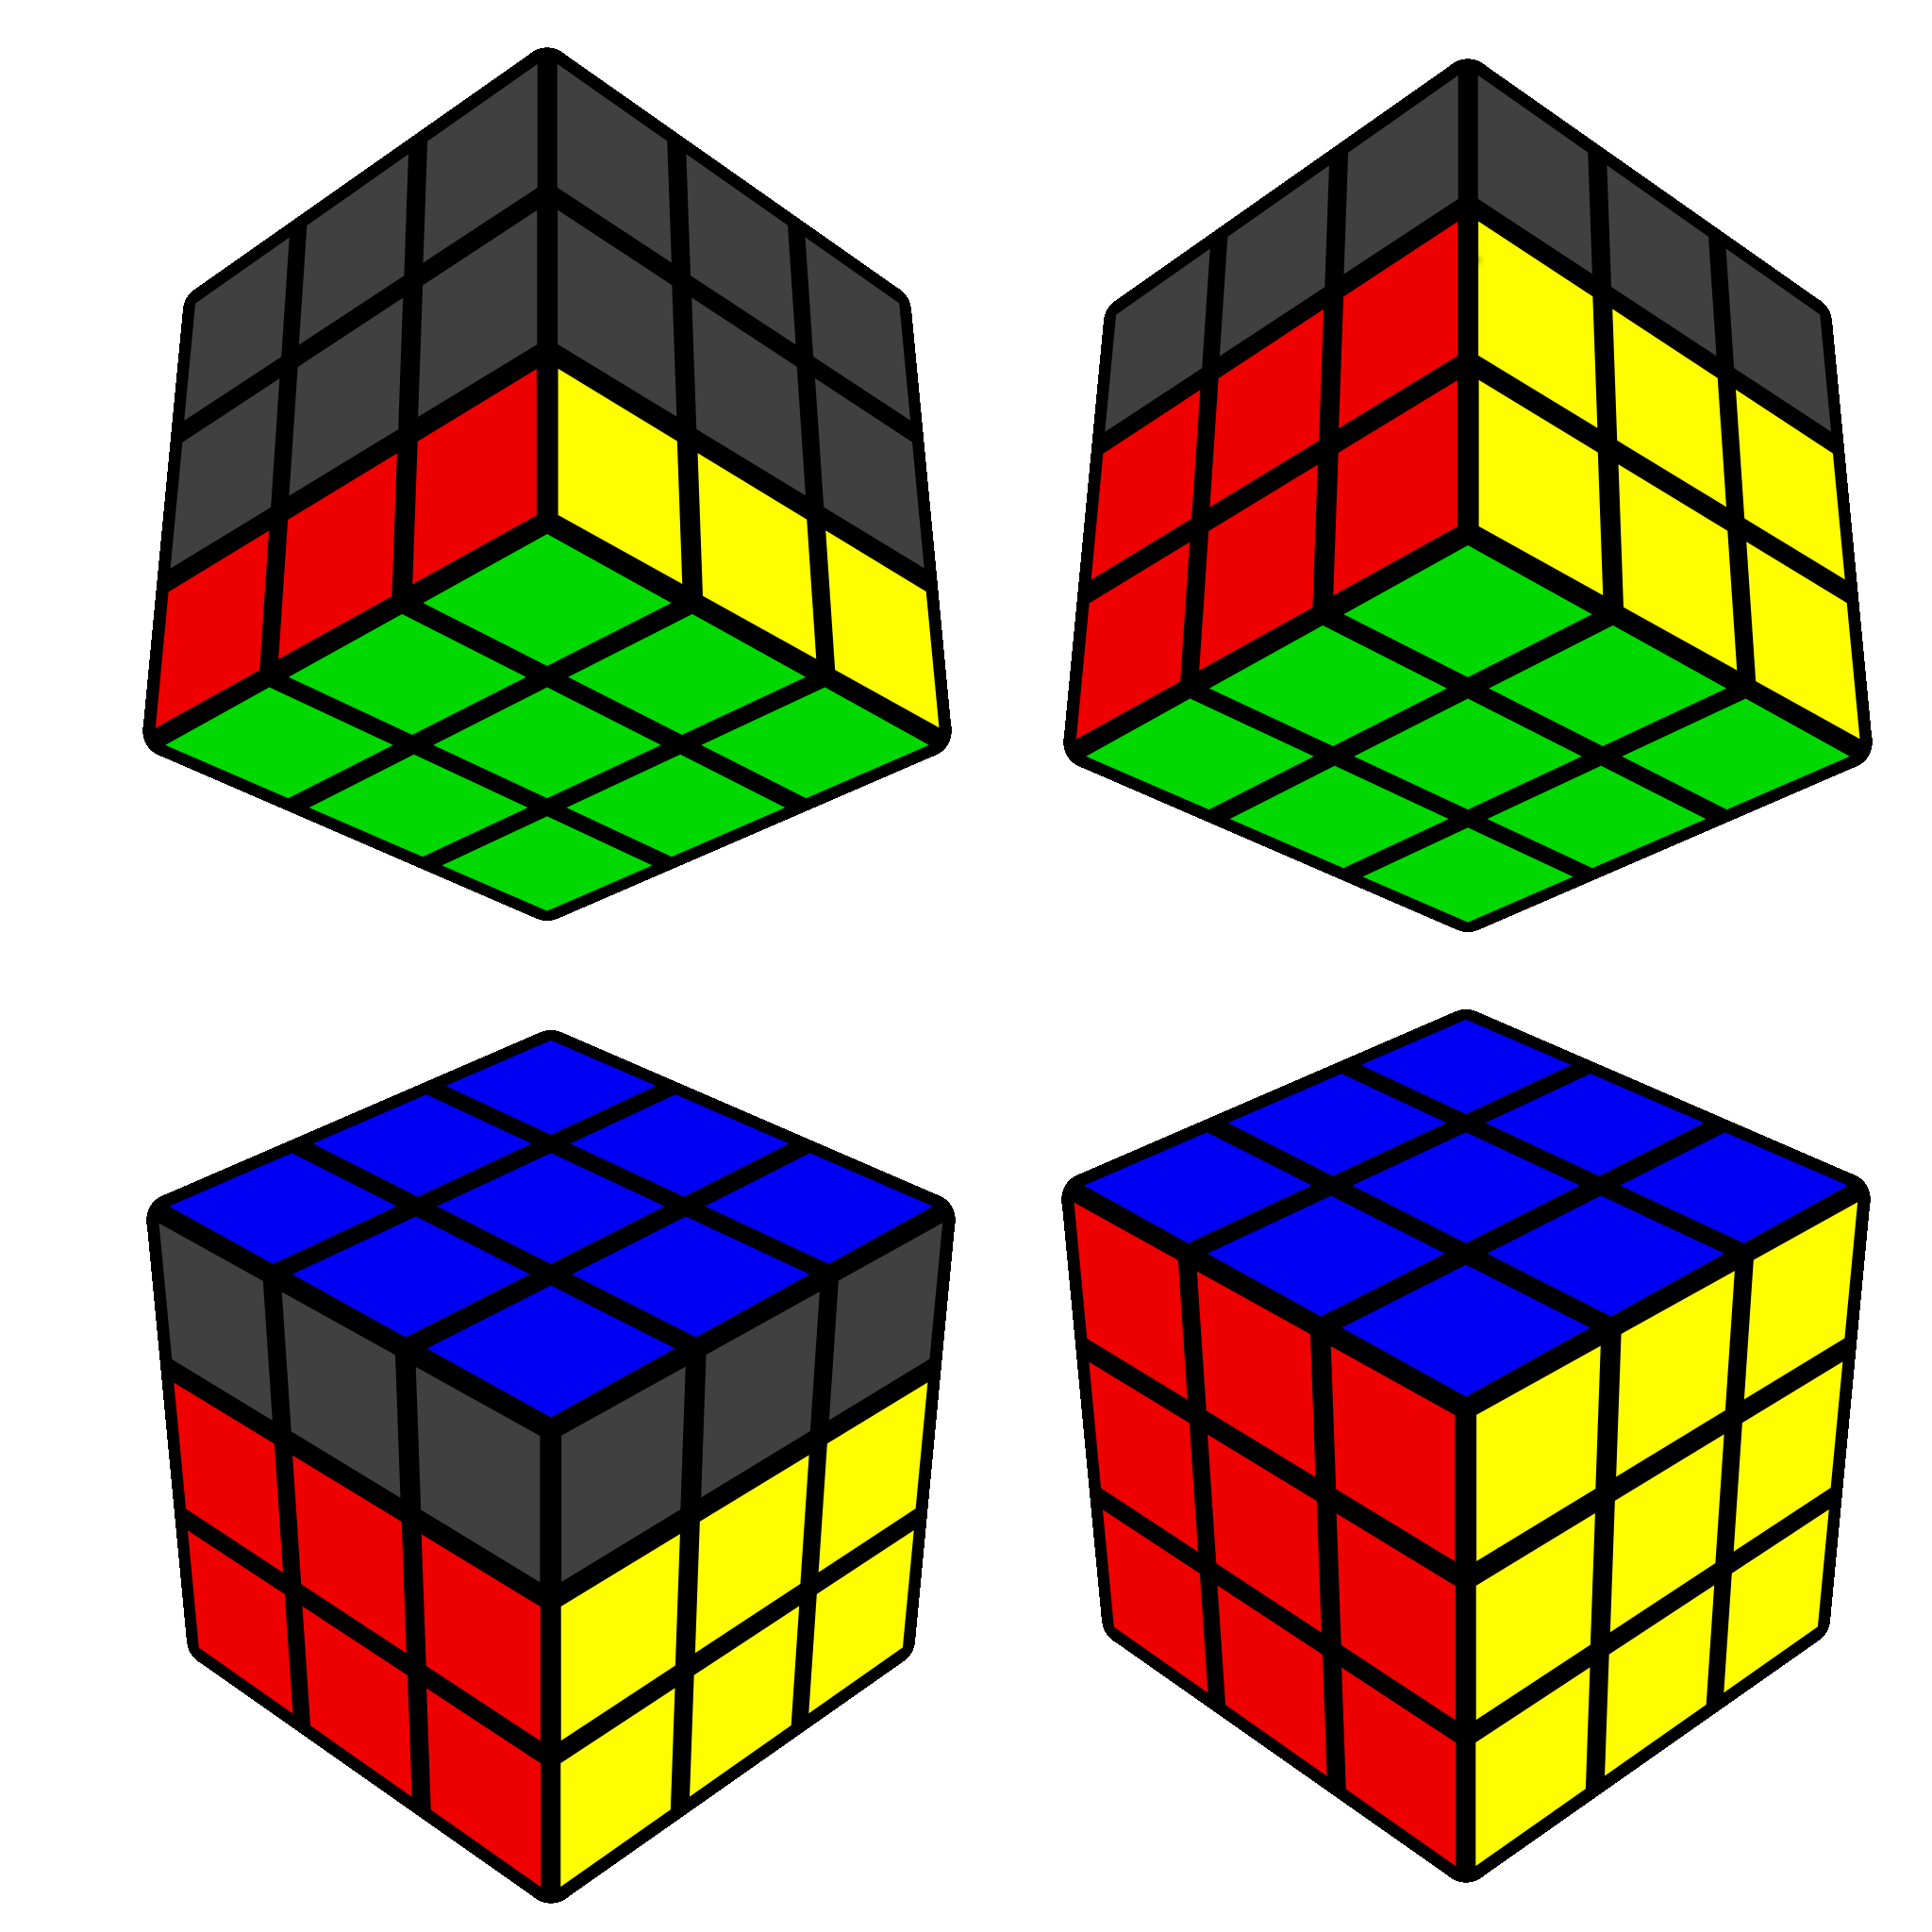
\includegraphics[width=0.3\textwidth]{union.png}
\caption*{The four steps of using the Layer by Layer Method}
\end{wrapfigure}
First off, I am going to cover the \emph{Beginner's Method}, also known as \emph{Layer by Layer Method} which does what the name implies: it solves the cube layer by layer. This method seems pretty intuitive to most people as it starts off by solving one Face (which is easy to begin with). The most common method is closely related to the Beginner's Method: \emph{Fridrich's Method} or more commonly known as \emph{CFOP} (I will admit, that name might sound very stange at first, yet it is justified). CFOP starts off by forming a \textbf{c}ross on one side, extending that cross to the \textbf{f}irst two layers, \textbf{o}rienting and \textbf{p}ermutating the last layer (leading to its unique name). You can see how closely related it is to the Beginner's Method: The key difference being that the Beginner's Method splits building the first two layers into two seperate steps whereas CFOP does this more efficiently. There are quite some more methods which deserve to be named here, for instance \emph{Petrus' Method}, but I'm going to leave it at that.


\section{Notation and terminology}
To be able to communicate on this abstract level of thinking, we are going to use the standart notation and terminology which I will explain below.

\chapter{Roux - theory}

\section{History}

\section{Idea}

\chapter{Roux - practical}

\section{First block}

\section{Second block}

\section{Corners Last Layer}

\section{Last six edges}

\chapter{Appendix: Algorithms}

\section{2 Look CLL}

\section{CMLL}

\section{LSE}


\end{document}